\documentclass[12pt]{examples/ai_conquer2026}
\addbibresource{examples/references.bib}
\graphicspath{{../figures/}}
\AIVNSetLogo{examples/Figures/logo.pdf}

% Biên dịch từ report/. Nhãn OWNER ghi rõ người phụ trách nội dung.
\newcommand{\owner}[1]{\textcolor{aivnGreen}{\textbf{Chủ mục: #1}}}

\title{%
  \begin{center}
    \Large {AI VIET NAM -- AI Conquer 2026}\\[.5ex]
    \Huge \textbf{So sánh mô hình dự đoán kết cục bệnh nhân gan}\\[.5ex]
    \large Hepatic Risk Outcome Prediction
  \end{center}
}
\posttitle{
  \author{
    \begin{minipage}{\textwidth}
      \centering
      {\vspace{-1.5em}Anh Tín (P1), Dương (P2), Nhất (P3), Anh Khôi (P4), Vân (P5)}
    \end{minipage}
  }
}
\date{}
\pagestyle{fancy}
\fancyhf{}
\lhead{\href{https://www.facebook.com/aivietnam.edu.vn}{\textcolor{aivnGreen}{\bfseries AI VIET NAM (AI Conquer 2026)}}}
\rhead{\href{https://aivietnam.edu.vn/}{\textcolor{aivnGreen}{\bfseries aivietnam.edu.vn}}}
\fancyfoot[C]{\thepage}
\renewcommand{\headrulewidth}{1.0pt}
\renewcommand{\headrule}{{\color{aivnGreen}\hrule width\headwidth height\headrulewidth \vskip-\headrulewidth}}

\begin{document}
\maketitle
\vspace{-5.5em}
\setlength{\epigraphwidth}{0.6\textwidth}

\section{Tóm tắt nghiên cứu}

Dự đoán xác suất kết cục của bệnh nhân gan là một bài toán dữ liệu bảng thuộc
Healthcare AI, trong đó chất lượng xác suất quan trọng không kém độ chính xác phân
loại. Bài toán gặp hai thách thức chính: nhãn mất cân bằng nghiêm trọng, với lớp
ghép gan CL chỉ chiếm khoảng 2.6\%, và nhiều đặc trưng lâm sàng, xét nghiệm có tỷ
lệ thiếu cao. Việc chỉ xếp hạng mô hình theo điểm trung bình chưa cho biết chênh
lệch có ổn định qua các fold hay xác suất có được calibration tốt hay không.
Nghiên cứu xây dựng một quy trình có thể tái lập để so sánh KNN, Logistic
Regression, Decision Tree, Naive Bayes, Random Forest và XGBoost trên 9.600 quan
sát có nhãn. Sau tiền xử lý, sáu mô hình được đánh giá trên cùng năm fold phân
tầng bằng log loss, accuracy và macro-F1. Chênh lệch log loss được phân tích bằng
kiểm định ghép cặp và hiệu chỉnh Bonferroni; mô hình tốt nhất tiếp tục được đánh
giá calibration trên dự đoán out-of-fold. XGBoost đạt kết quả tốt nhất với log
loss $0.382\pm0.007$, accuracy $0.850\pm0.006$ và macro-F1 $0.640\pm0.032$.
Sau hiệu chỉnh, XGBoost tốt hơn Random Forest, Decision Tree, KNN và Naive Bayes;
với Logistic Regression, bằng chứng chưa đủ theo exact Wilcoxon. XGBoost đạt
top-label ECE 0.0117 và multiclass Brier score 0.2162. Đóng góp chính của nghiên
cứu là protocol dùng chung fold, kết hợp đánh giá hiệu năng, suy diễn thống kê,
calibration, ablation và pipeline submission có kiểm soát schema và provenance.

\newpage
\setcounter{tocdepth}{2}
\tableofcontents
\thispagestyle{fancy}
\newpage

\section{Giới thiệu (Introduction)}

Dự đoán kết cục của bệnh nhân mắc bệnh gan là một bài toán dữ liệu bảng thuộc
lĩnh vực Healthcare AI. Thông tin sẵn có cho mỗi bệnh nhân không chỉ bao gồm tuổi
và giới tính mà còn có thời gian theo dõi, chỉ định điều trị, giai đoạn lâm sàng,
các dấu hiệu như cổ trướng, gan to, phù và sao mạch, cùng nhiều chỉ số xét nghiệm.
Việc khai thác đồng thời những nguồn thông tin này có thể hỗ trợ mô hình nhận diện
các mẫu liên quan đến diễn tiến bệnh. Tuy nhiên, kết quả của nghiên cứu này chỉ là
đánh giá phương pháp học máy trên dữ liệu cuộc thi, không phải công cụ chẩn đoán
hay khuyến nghị điều trị trong thực hành lâm sàng.

Nhiệm vụ của AIO 2026-1 Hepatic Risk Outcome Prediction yêu cầu mô hình ước lượng
xác suất cho ba kết cục: bệnh nhân còn sống hoặc bị kiểm duyệt theo dõi (C), bệnh
nhân được ghép gan và bị kiểm duyệt (CL), hoặc tử vong (D). Đây không đơn thuần là
bài toán chọn một nhãn. Đầu ra phải là một phân phối xác suất hợp lệ, vì hệ thống
đánh giá bằng multiclass log loss. Một dự đoán sai với độ tự tin cao bị phạt mạnh
hơn nhiều so với một dự đoán sai nhưng còn thể hiện độ bất định. Do đó, nghiên cứu
cần xem xét đồng thời khả năng phân loại, chất lượng xác suất và calibration.

Bộ dữ liệu đặt ra ba khó khăn chính. Thứ nhất, phân bố nhãn mất cân bằng rõ rệt:
lớp C chiếm khoảng 67.9\%, lớp D khoảng 29.4\%, còn lớp CL chỉ khoảng 2.6\%. Một
mô hình thiên về lớp phổ biến vẫn có thể đạt accuracy tương đối cao nhưng hoạt
động kém trên lớp hiếm. Thứ hai, nhiều biến lâm sàng và xét nghiệm bị thiếu với tỷ
lệ lớn; riêng \texttt{Edema\_Status} thiếu khoảng 92\%, trong khi Cholesterol và
Triglyceride thiếu khoảng 55\%. Thứ ba, nhiều chỉ số xét nghiệm lệch phải và khác
nhau đáng kể về thang đo, làm cho tiền xử lý có ảnh hưởng trực tiếp đến các mô hình
nhạy với khoảng cách hoặc regularization.

Trong bối cảnh đó, chỉ so sánh điểm trung bình của nhiều mô hình là chưa đủ. Một
chênh lệch quan sát được có thể xuất phát từ một cách chia train--validation cụ
thể, trong khi các mô hình lại được đánh giá trên cùng bệnh nhân ở từng fold. Dự
án vì vậy tập trung vào phương pháp luận so sánh: sử dụng cùng năm fold phân tầng,
tính cùng bộ chỉ số, thực hiện kiểm định ghép cặp trên chênh lệch theo fold, báo
cáo khoảng tin cậy và kiểm soát sai số do so sánh nhiều mô hình. Ngoài hiệu năng,
nghiên cứu còn đánh giá calibration của mô hình tốt nhất bằng reliability diagram,
expected calibration error và Brier score.

Mục tiêu tổng quát của nghiên cứu là xây dựng một quy trình có thể tái lập để so
sánh sáu họ mô hình --- KNN, Logistic Regression, Decision Tree, Naive Bayes,
Random Forest và XGBoost --- trên cùng dữ liệu và cùng protocol. Quy trình bao phủ
từ phân tích dữ liệu, tiền xử lý, cố định fold, huấn luyện, đánh giá thống kê đến
tạo file submission. Qua đó, nghiên cứu hướng tới một kết luận thận trọng hơn câu
hỏi ``mô hình nào có điểm thấp nhất'': kết quả tốt hơn bao nhiêu, có ổn định qua
fold hay không, xác suất có đáng tin cậy hay không, và toàn bộ kết quả có thể được
truy vết tới artifact nguồn hay không.

\subsection{Đóng góp}

Nghiên cứu có năm đóng góp chính:

\begin{itemize}
\item \textbf{Xây dựng pipeline dữ liệu thống nhất và có thể kiểm tra.} Dữ liệu
được tổ chức theo ba tầng \texttt{raw}, \texttt{interim} và \texttt{processed};
pipeline xử lý dữ liệu thiếu, bổ sung cờ missing, encode biến phân loại, biến đổi
\texttt{log1p} cho biến lệch phải và lưu đồng thời phiên bản có/không scaling.

\item \textbf{Thiết lập protocol so sánh công bằng cho sáu mô hình.} Năm fold
phân tầng với seed 42 được tạo một lần và dùng chung cho mọi model track. Nhờ đó,
điểm của các mô hình được ghép đúng theo cùng fold, tránh việc so sánh các kết quả
đến từ những lần chia dữ liệu khác nhau.

\item \textbf{Đánh giá thực nghiệm đa chiều.} Sáu mô hình thuộc ba track được so
sánh bằng log loss, accuracy và macro-F1. Nghiên cứu bổ sung ablation về ảnh hưởng
của scaling đối với KNN và Logistic Regression, đồng thời phân tích sự khác biệt
giữa cây đơn không regularization, cây giới hạn độ sâu, Random Forest và XGBoost.

\item \textbf{Bổ sung tầng suy diễn thống kê và calibration.} Chênh lệch log loss
được phân tích bằng kiểm định ghép cặp, Shapiro--Wilk, exact Wilcoxon khi giả định
chuẩn không phù hợp, khoảng tin cậy và hiệu chỉnh Bonferroni cho năm phép so sánh.
Mô hình tốt nhất còn được đánh giá bằng top-label ECE, classwise ECE, Brier score
và phân tích độ nhạy theo số bin.

\item \textbf{Hoàn thiện quy trình submission và provenance.} Module tạo file
nộp kiểm tra số dòng, ID trùng, thứ tự lớp, giá trị NaN/vô hạn, miền xác suất và
tổng xác suất theo dòng trước khi ghi CSV. Các bảng, hình, OOF prediction, manifest
và kết quả validation được lưu thành artifact để con số trong báo cáo có thể truy
vết và tái tạo.
\end{itemize}

\section{Bài toán nghiên cứu (Research Problem)}

Nghiên cứu được xác định tường minh như sau:

\begin{itemize}
\item \textbf{Tên bài toán:} Phân loại đa lớp trên dữ liệu bảng
(tabular multiclass classification) để dự đoán xác suất kết cục của bệnh nhân gan.

\item \textbf{Input:} Một vector đặc trưng cho mỗi bệnh nhân, gồm thông tin nhân
khẩu học, thời gian theo dõi, chỉ định điều trị, giai đoạn lâm sàng, dấu hiệu lâm
sàng và các chỉ số xét nghiệm. Cột \texttt{id} chỉ dùng để định danh và không được
dùng làm đặc trưng dự đoán.

\item \textbf{Output:} Vector gồm ba xác suất tương ứng với C (còn sống hoặc bị
kiểm duyệt theo dõi), CL (được ghép gan và bị kiểm duyệt) và D (tử vong). Ba xác
suất phải thuộc $[0,1]$ và có tổng bằng một.

\item \textbf{Mục tiêu nghiên cứu:} So sánh sáu mô hình học máy trên cùng protocol
5-fold, tìm mô hình có log loss thấp và ổn định, kiểm tra ý nghĩa thống kê của
chênh lệch, đánh giá calibration, đồng thời xây dựng quy trình có thể tái lập từ
dữ liệu thô đến submission.

\item \textbf{Metric đánh giá:} Multiclass log loss là metric chính; accuracy và
macro-F1 là metric bổ trợ. Calibration được đánh giá bằng reliability diagram,
expected calibration error (ECE) và multiclass Brier score. Runtime được ghi nhận
để mô tả chi phí huấn luyện và suy luận trong môi trường thí nghiệm.
\end{itemize}

\subsection{Định nghĩa input và output}

Gọi $\mathbf{x}_i\in\mathcal{X}$ là vector đặc trưng của bệnh nhân thứ $i$. Sau
khi loại cột định danh và thực hiện feature engineering, vector này được hình thành
từ bốn nhóm thông tin: (1) nhân khẩu học; (2) thời gian theo dõi, điều trị và giai
đoạn lâm sàng; (3) dấu hiệu lâm sàng; và (4) chỉ số xét nghiệm. Nhãn đích là
$y_i\in\mathcal{Y}=\{C,CL,D\}$.

Mô hình $f_{\theta}:\mathcal{X}\rightarrow\Delta^2$ ánh xạ mỗi bệnh nhân thành
một vector xác suất
\[
\hat{\mathbf p}_i=f_{\theta}(\mathbf{x}_i)
=(\hat p_{i,C},\hat p_{i,CL},\hat p_{i,D}),
\]
trong đó $0\leq\hat p_{i,k}\leq1$ và
$\hat p_{i,C}+\hat p_{i,CL}+\hat p_{i,D}=1$. Khi nộp bài, vector này được ghi theo
đúng schema \texttt{id, Status\_C, Status\_CL, Status\_D}. Thứ tự lớp phải được
giữ cố định xuyên suốt quá trình encode nhãn, gọi \texttt{predict\_proba}, tính
metric và tạo submission.

\subsection{Mục tiêu tối ưu và tiêu chí đánh giá}

Metric chính là multiclass log loss:
\[
\mathcal L=-\frac{1}{N}\sum_{i=1}^{N}
\sum_{k\in\{C,CL,D\}}y_{ik}\log(\hat p_{i,k}),
\]
trong đó $y_{ik}=1$ nếu quan sát $i$ thuộc lớp $k$ và bằng 0 trong các trường hợp
còn lại. Log loss càng thấp càng tốt. Do logarit tiến tới âm vô cùng khi xác suất
tiến về 0, metric này phạt đặc biệt mạnh trường hợp mô hình gán xác suất gần 0 cho
nhãn thực. Đặc tính đó phù hợp với yêu cầu của cuộc thi nhưng cũng khiến các mô
hình sinh xác suất cực đoan, như cây đơn quá sâu hoặc KNN với ít láng giềng, dễ có
kết quả rất kém.

Accuracy được báo cáo để thể hiện tỷ lệ dự đoán đúng theo lớp có xác suất cao nhất.
Macro-F1 tính F1 riêng cho từng lớp rồi lấy trung bình không trọng số, nhờ đó phản
ánh tốt hơn hiệu năng trên lớp CL hiếm. Hai chỉ số này là metric bổ trợ; quyết định
mô hình cuối vẫn dựa trước hết vào log loss. Với mô hình có log loss thấp nhất,
nghiên cứu tiếp tục đánh giá calibration bằng ECE và Brier score để phân biệt giữa
khả năng xếp đúng lớp và độ tin cậy của xác suất.

\subsection{Thiết kế đánh giá}

Tập train dùng cho đánh giá chính gồm 9.600 bệnh nhân có nhãn; tập test gồm 10.000 bệnh nhân không có
nhãn. Đánh giá nội bộ sử dụng Stratified 5-Fold cố định, mỗi quan sát xuất hiện
đúng một lần trong validation và bốn lần trong phần huấn luyện. Mọi mô hình dùng
chung \texttt{fold\_id}; vì vậy chênh lệch log loss ở fold $j$ được định nghĩa là
\[
d_j=\mathcal L_{\mathrm{XGB},j}-\mathcal L_{\mathrm{comparator},j}.
\]
Giá trị $d_j<0$ nghiêng về XGBoost. Năm comparator tạo thành một family kiểm định;
p-value được hiệu chỉnh Bonferroni với family-wise $\alpha=0.05$. Thiết kế này
giúp trả lời liệu lợi thế quan sát được có nhất quán trên cùng các fold hay không,
nhưng không loại bỏ hoàn toàn sự phụ thuộc do các tập training giữa fold chồng lấp.

\subsection{Câu hỏi và giả thuyết nghiên cứu}

\begin{itemize}
\item \textbf{RQ1:} Trong sáu mô hình được khảo sát, mô hình nào đạt mean 5-fold
log loss thấp nhất, đồng thời duy trì accuracy và macro-F1 cạnh tranh?
\item \textbf{RQ2:} Chênh lệch log loss giữa mô hình đứng đầu và từng comparator
có đủ bằng chứng thống kê sau khi kiểm tra giả định và hiệu chỉnh năm phép so sánh
hay không?
\item \textbf{RQ3:} Scaling ảnh hưởng như thế nào đến KNN và Logistic Regression,
và regularization/ensemble ảnh hưởng như thế nào đến độ cực đoan của xác suất cây?
\item \textbf{RQ4:} Xác suất out-of-fold của mô hình tốt nhất có calibration tốt
không, và kết luận ECE có ổn định khi thay đổi số bin hay không?
\end{itemize}

\begin{aivncodebox}[Giả thuyết nghiên cứu]
H1: Các ensemble cây, đặc biệt XGBoost có regularization, đạt log loss
thấp hơn Decision Tree đơn vì giảm phương sai và hạn chế xác suất quá tự tin.

H2: Scaling cải thiện hiệu năng của KNN vì khoảng cách không còn bị chi
phối bởi các đặc trưng có đơn vị và miền giá trị lớn.

H3: Xác suất out-of-fold của mô hình có log loss thấp nhất có sai lệch
calibration nhỏ và kết luận ECE tương đối ổn định khi thay đổi số bin.
\end{aivncodebox}

Các giả thuyết được đánh giá trên validation 5-fold. Kết quả leaderboard, nếu có,
chỉ đóng vai trò đối chiếu ngoài mẫu và không được dùng hồi tố để thay đổi protocol
nghiên cứu.

\section{Tổng quan nghiên cứu liên quan (Related Work)}
\owner{Vân (P5) viết và tích hợp; Anh Tín (P1), Dương (P2), Nhất (P3) và Anh Khôi
(P4) duyệt phần liên quan đến track của mình.}

\subsection{Dự đoán tiên lượng bệnh gan}

Nghiên cứu tiên lượng bệnh gan có lịch sử lâu hơn các benchmark phân loại hiện
đại. Dickson và cộng sự xây dựng mô hình Cox từ dữ liệu bệnh nhân xơ gan mật
nguyên phát tại Mayo Clinic, sử dụng tuổi, bilirubin, albumin, thời gian
prothrombin và mức độ phù để dự đoán sống còn. Mô hình được kiểm tra trên một tập
bệnh nhân độc lập và có ưu điểm không yêu cầu sinh thiết gan
\cite{dickson1989prognosis}. Công trình này cho thấy các biến lâm sàng và xét
nghiệm dạng bảng có thể mang tín hiệu tiên lượng hữu ích, đồng thời nhấn mạnh vai
trò của đánh giá ngoài mẫu.

Một benchmark liên quan trực tiếp là Cirrhosis Patient Survival Prediction trong
UCI Machine Learning Repository. Bộ dữ liệu có 418 bệnh nhân, 17 đặc trưng và ba
trạng thái D, C, CL; dữ liệu bắt nguồn từ nghiên cứu Mayo Clinic giai đoạn
1974--1984 \cite{dickson1989uci}. Bộ dữ liệu của cuộc thi hiện tại có cấu trúc biến
và định nghĩa nhãn tương tự. Gói dữ liệu hiện có gồm 9.600 quan sát train, 2.400
quan sát validation riêng và 10.000 quan sát test.
Do ban tổ chức không cung cấp trong repo một tài liệu mô tả chính thức về quy trình
mở rộng dữ liệu, nghiên cứu này không giả định rằng hai bộ dữ liệu hoàn toàn giống
nhau và không dùng kết quả trên UCI làm benchmark số trực tiếp.

\subsection{Các mô hình học máy truyền thống}

Các phương pháp truyền thống cung cấp những baseline với giả định khác nhau.
Logistic Regression mô hình hóa log-odds tuyến tính, huấn luyện nhanh và tạo xác
suất trực tiếp, nhưng có thể bỏ sót quan hệ phi tuyến hoặc tương tác phức tạp. KNN
không giả định dạng hàm và tận dụng cấu trúc cục bộ, song nhạy với scaling, nhiễu,
chiều dữ liệu và lựa chọn số láng giềng. Naive Bayes có chi phí thấp nhưng giả định
độc lập có điều kiện thường không phù hợp hoàn toàn với các chỉ số xét nghiệm có
tương quan. Decision Tree dễ diễn giải và học được ngưỡng phi tuyến, nhưng cây sâu
có phương sai lớn và thường tạo xác suất 0 hoặc 1 ở các lá ít mẫu. Trong bài toán
dùng log loss, nhược điểm sau đặc biệt nghiêm trọng vì một dự đoán sai với xác suất
gần 0 cho nhãn thực sẽ bị phạt rất mạnh.

Những mô hình này vẫn cần thiết ngay cả khi ensemble đạt kết quả cao hơn. Chúng tạo
ra mốc so sánh về độ phức tạp, tốc độ và giả định mô hình; đồng thời giúp xác định
lợi ích của từng thành phần. Dự án kế thừa cách tiếp cận baseline đa dạng này và
bổ sung ablation có/không scaling cho KNN và Logistic Regression, cũng như so sánh
cây không giới hạn độ sâu với cây đã regularize.

\subsection{Ensemble cây và mô hình hiện đại cho dữ liệu bảng}

Random Forest kết hợp nhiều cây được huấn luyện trên bootstrap samples và sử dụng
ngẫu nhiên đặc trưng tại mỗi nút. Breiman chỉ ra rằng sai số tổng quát phụ thuộc
vào sức mạnh của từng cây và tương quan giữa chúng; việc averaging giúp mô hình
ổn định hơn cây đơn và tương đối bền vững trước nhiễu \cite{breiman2001random}.
Hạn chế của Random Forest là nhiều cây có thể làm tăng chi phí suy luận, còn xác
suất trung bình không mặc nhiên bảo đảm calibration tối ưu.

XGBoost xây dựng cây tuần tự để sửa sai của ensemble hiện tại, kết hợp regularized
objective, shrinkage, subsampling và các tối ưu cho dữ liệu thưa. Công trình gốc
mô tả một hệ thống tree boosting có khả năng mở rộng và đạt kết quả mạnh trong
nhiều thử thách học máy \cite{chen2016xgboost}. Với dữ liệu bảng có quan hệ phi
tuyến, tương tác và missingness, gradient-boosted trees thường là ứng viên phù hợp;
tuy nhiên, hiệu năng phụ thuộc vào siêu tham số và việc dùng cùng fold để tuning
và đánh giá có thể tạo selection bias.

Các kiến trúc deep learning và pretrained/foundation models không phải trọng tâm
của nghiên cứu này. Dataset là dữ liệu bảng kích thước vừa, không có ảnh, văn bản
hay tín hiệu tuần tự cần representation learning từ mô hình tiền huấn luyện. Việc
thêm mạng sâu mà không có protocol tuning tương xứng sẽ làm tăng không gian thử
nghiệm và giảm khả năng diễn giải. Vì vậy, phạm vi được chủ động giới hạn ở sáu mô
hình học máy đại diện để tập trung vào phương pháp so sánh và chất lượng xác suất.

\subsection{Đánh giá xác suất và so sánh thống kê}

Accuracy chỉ đánh giá lớp có xác suất lớn nhất và không phân biệt dự đoán đúng với
độ tự tin 0.51 hay 0.99. Log loss và Brier score đánh giá toàn bộ phân phối xác
suất; Brier score bắt nguồn từ nghiên cứu về kiểm chứng dự báo xác suất
\cite{brier1950verification}. Reliability diagram và ECE đo khoảng cách giữa mức
confidence và tần suất đúng quan sát được. Guo và cộng sự cho thấy mô hình có
accuracy tốt vẫn có thể calibration kém và temperature scaling là một baseline
hậu xử lý hiệu quả trong nhiều thiết lập \cite{guo2017calibration}. Dù công trình
đó tập trung vào mạng nơ-ron, kết luận khái quát rằng hiệu năng phân loại và
calibration là hai khía cạnh khác nhau vẫn phù hợp với nghiên cứu này.

So sánh nhiều mô hình cũng làm phát sinh nguy cơ kết luận dương tính giả nếu thực
hiện nhiều kiểm định mà không hiệu chỉnh. Demšar tổng hợp các phương pháp so sánh
classifier và khuyến nghị các kiểm định phi tham số như Wilcoxon trong những thiết
lập phù hợp, đồng thời nhấn mạnh vấn đề multiple comparisons
\cite{demsar2006statistical}. Dự án kế thừa nguyên tắc kiểm định ghép cặp và kiểm
soát family-wise error, nhưng chỉ có năm fold trên một dataset; vì vậy độ phân giải
của kiểm định thấp và các fold không thể được xem như năm dataset độc lập.

\subsection{Khoảng trống và định vị nghiên cứu}

Từ các hướng nghiên cứu trên, bốn khoảng trống được xác định trong phạm vi project:

\begin{itemize}
\item Chưa có một baseline thống nhất so sánh sáu họ mô hình trên đúng bộ dữ liệu
cuộc thi bằng cùng fold và cùng cách tính metric.
\item Ảnh hưởng của scaling đối với mô hình dựa trên khoảng cách và ảnh hưởng của
regularization/ensemble đối với xác suất cây chưa được tách bằng ablation rõ ràng.
\item Xếp hạng theo mean log loss chưa trả lời chênh lệch có nhất quán qua fold và
còn tồn tại sau hiệu chỉnh so sánh bội hay không.
\item Mô hình tốt nhất theo log loss vẫn cần được kiểm tra calibration, độ nhạy
theo số bin và provenance của dự đoán out-of-fold.
\end{itemize}

Nghiên cứu này không tuyên bố một kiến trúc mới. Đóng góp nằm ở việc kiểm chứng và
tích hợp: xây dựng baseline có thể tái lập, đánh giá sáu mô hình trên shared
5-fold, thực hiện hai ablation có mục tiêu, kết hợp suy diễn thống kê với phân tích
calibration, và duy trì artifact từ dữ liệu tới submission. Các nội dung này trực
tiếp hỗ trợ RQ1--RQ4 đã nêu ở phần Bài toán nghiên cứu và tạo cơ sở cho phân tích
lỗi, giới hạn cùng hướng phát triển ở các phần sau.

\section{Phương pháp nghiên cứu (Methodology)}
\owner{Anh Tín (P1) phụ trách dữ liệu và Track C; Dương (P2) Track A; Nhất (P3)
Track B; Anh Khôi (P4) thống kê; Vân (P5) tích hợp.}

\subsection{Pipeline dữ liệu}

Quy trình được tổ chức theo ba tầng
\texttt{raw $\rightarrow$ interim $\rightarrow$ processed}. Tầng raw giữ nguyên
CSV do ban tổ chức cung cấp. Ở tầng interim, nhóm chuyển
\texttt{Patient\_Age\_Days} thành tuổi theo năm, loại \texttt{Edema\_Status} do
thiếu khoảng 92\% nhưng giữ một cờ biểu thị missingness, và tạo thêm cờ thiếu cho
các biến có tỷ lệ thiếu cao. Biến số được điền bằng median tính trên train; biến
phân loại thiếu được gán nhãn \texttt{Unknown}. ID và fold ID không được đưa vào
tập đặc trưng.

Ở tầng processed, sáu biến lệch phải gồm Bilirubin, Cholesterol, Copper, Alkaline
Phosphatase, AST và Triglyceride được biến đổi \texttt{log1p}. Nhóm tạo thêm tỷ lệ
Bilirubin/Albumin rồi cũng áp dụng \texttt{log1p}. Các biến phân loại được mã hóa
bằng \texttt{OrdinalEncoder}; giá trị chưa từng thấy ở test nhận mã $-1$. Đặc
trưng số được scale bằng \texttt{RobustScaler}, phù hợp hơn StandardScaler khi có
outlier. Pipeline tạo 31 đặc trưng cuối cùng và lưu thêm một phiên bản không scale
có cùng cột, cùng encoding và cùng biến đổi để thực hiện ablation.

Một giới hạn cần công khai là median, encoder và scaler hiện được fit một lần trên
toàn bộ 9.600 dòng train trước khi chạy cross-validation, thay vì được fit riêng
trong từng training fold. Cách làm này không dùng nhãn validation nhưng vẫn cho
phép thống kê phân phối của validation đi vào tiền xử lý, tạo leakage nhẹ và có
thể làm score hoặc calibration lạc quan. Báo cáo giữ nguyên artifact đã freeze và
đưa vấn đề này vào phần hạn chế; phiên bản tiếp theo cần dùng
\texttt{Pipeline}/\texttt{ColumnTransformer} bên trong từng fold.

\subsection{Thiết kế validation dùng chung}

Nhóm tạo Stratified 5-Fold với \texttt{shuffle=True} và seed 42, sau đó lưu cố
định tại \texttt{data/interim/fold\_id.csv}. Mỗi fold có 1.920 mẫu; fold 0 gồm
1.305 C, 50 CL và 565 D, còn mỗi fold 1--4 gồm 1.304 C, 51 CL và 565 D. Toàn bộ
9.600 ID train là duy nhất. Mọi model track dùng cùng fold ID và huấn luyện lại
mô hình từ đầu ở mỗi fold; điều này tạo các cặp điểm hợp lệ cho so sánh thống kê.
Không có oversampling, class weighting hay dữ liệu test trong quá trình đánh giá.

\subsection{Các mô hình và quy tắc chọn cấu hình}

\subsubsection{Track A: KNN và Logistic Regression}
\owner{Dương (P2).}

KNN được quét \texttt{n\_neighbors} trong
$\{3,5,7,9,11,15,21,31,41,51\}$ trên shared 5-fold và chọn theo mean log loss;
$k=51$ là cấu hình tốt nhất. Các tham số còn lại dùng mặc định của
scikit-learn: uniform weights và khoảng cách Minkowski với $p=2$ (Euclid).
Logistic Regression dùng regularization L2 mặc định, $C=1$, solver mặc định
\texttt{lbfgs}, \texttt{max\_iter=1000} và seed 42. Cả hai nhận bản dữ liệu đã
scale. Bản không scale chỉ dùng cho ablation và không tham gia bảng xếp hạng cuối.

\subsubsection{Track B: Decision Tree và Naive Bayes}
\owner{Nhất (P3).}

Decision Tree được quét \texttt{max\_depth} trong
$\{2,3,4,5,6,8,10,12,15,20,\mathrm{None}\}$ và chọn độ sâu 3 theo mean log loss.
Mô hình dùng criterion Gini, \texttt{min\_samples\_leaf=1} và seed 42. Baseline
thứ hai là \texttt{GaussianNB} với \texttt{var\_smoothing=$10^{-9}$} mặc định.
Project không clip xác suất ở tầng metric; \texttt{sklearn.log\_loss} tự bảo vệ
phép log ở machine epsilon. Quyết định này giúp ablation phản ánh đúng hậu quả của
xác suất 0 do cây không giới hạn độ sâu.

\subsubsection{Track C: Random Forest và XGBoost}
\owner{Anh Tín (P1).}

Random Forest được grid search trên \texttt{n\_estimators} $\in\{200,400,600\}$
và \texttt{max\_depth} $\in\{6,8,10,14,\mathrm{None}\}$. Cấu hình freeze là 600
cây, độ sâu 14, seed 42 và chạy song song với \texttt{n\_jobs=-1}. XGBoost được
quét 200/400 cây, độ sâu 2--6 và learning rate
$\{0.03,0.05,0.10,0.15,0.20\}$; cấu hình freeze là 400 cây, độ sâu 2 và learning
rate 0.15. Mô hình dùng \texttt{eval\_metric=mlogloss}, seed 42 và các giá trị
mặc định cho subsample/column sampling. Không sử dụng early stopping hay class
weights. Sau khi freeze, hai mô hình được chạy lại trên cùng năm fold để tạo bảng
điểm cuối và OOF prediction.

\subsection{Phân tích thống kê và calibration}
\owner{Anh Khôi (P4).}

XGBoost được chọn làm mô hình tham chiếu sau khi có mean log loss thấp nhất. Với
mỗi comparator, nhóm tính năm chênh lệch ghép cặp
$d_j=\mathcal L_{\mathrm{XGB},j}-\mathcal L_{\mathrm{comp},j}$. Shapiro--Wilk
được dùng như cổng chọn primary test: paired t-test nếu $p\geq0.05$, exact
Wilcoxon hai phía nếu $p<0.05$. Năm phép so sánh được hiệu chỉnh Bonferroni với
family-wise $\alpha=0.05$, nên adjusted alpha là 0.01. T-based 95\% CI được báo
cáo như đại lượng mô tả cho chênh lệch trung bình; kết luận chính dựa trên primary
test. Với XGBoost, OOF prediction chỉ được dùng cho calibration sau khi cổng tái
tạo xác nhận metric khớp score theo cả năm fold. Calibration được mô tả bằng
reliability diagram, top-label ECE, macro classwise ECE, multiclass Brier score và
phân tích độ nhạy với 5, 10, 15, 20 bins.

\section{Dữ liệu và thiết lập thí nghiệm (Experiments)}
\owner{Anh Tín (P1) dữ liệu; các model owner xác nhận cấu hình.}

\subsection{Dataset và chia dữ liệu}

Gói dữ liệu gồm \texttt{aio26\_train.csv} (9.600 dòng, 18 đặc trưng, ID và nhãn),
\texttt{aio26\_val.csv} (2.400 dòng có nhãn), \texttt{aio26\_test.csv} (10.000
dòng không nhãn) và sample submission. Phân tích chính và toàn bộ bảng so sánh
thống kê trong báo cáo được tạo từ 9.600 dòng train trên shared 5-fold; file val
riêng không được gộp vào các điểm này. Test chỉ dùng để sinh submission và không
được dùng trong tuning hay đánh giá.

Trong train, C có 6.521 mẫu (67.93\%), D có 2.825 mẫu (29.43\%), CL có 254 mẫu
(2.65\%). Các fold được phân tầng gần như đồng nhất: mỗi fold có 1.920 mẫu, gồm
50--51 CL, 565 D và 1.304--1.305 C; mỗi lượt huấn luyện dùng 7.680 mẫu và đánh giá
trên 1.920 mẫu còn lại.

\begin{figure}[H]
\centering
\includegraphics[width=.92\linewidth]{eda/fig1_overview_dashboard.png}
\caption{Tổng quan kích thước, phân bố nhãn và tỷ lệ thiếu trên tập train 9.600 mẫu.}
\label{fig:eda}
\end{figure}

EDA cho thấy \texttt{Edema\_Status} thiếu 92.01\%, Triglyceride và Cholesterol
thiếu lần lượt 55.66\% và 55.35\%; nhiều biến điều trị, dấu hiệu và xét nghiệm
thiếu khoảng 43\%. Bilirubin, Alkaline Phosphatase, Copper, Cholesterol và một số
xét nghiệm lệch phải rõ rệt. So sánh histogram mật độ của tám biến chính giữa
train và test không cho thấy dịch chuyển phân phối nổi bật bằng quan sát trực quan.
Tuy nhiên, notebook chưa thực hiện một kiểm định drift định lượng hoặc đặt ngưỡng
phát hiện trước, nên kết quả này chỉ là chẩn đoán EDA, không phải bằng chứng rằng
hai phân phối hoàn toàn giống nhau.

\subsection{Thiết lập huấn luyện và đánh giá}

Môi trường authoritative được ghi trong \texttt{requirements.lock.txt}: Python
3.9.18, XGBoost 2.1.4, scikit-learn 1.6.1, NumPy 1.26.4, pandas 2.3.3, SciPy
1.13.1 và Matplotlib 3.9.2. Seed thống nhất là 42. Notebook không ghi model CPU,
RAM hoặc GPU, vì vậy runtime chỉ mô tả lần chạy hiện tại và không được diễn giải
như benchmark phần cứng.

Mỗi mô hình được clone và fit lại từ đầu trên từng training fold. Hàm metric dùng
cùng thứ tự nhãn $[0,1,2]$ để tránh lỗi khi lớp hiếm ít xuất hiện. Log loss là
metric chọn cấu hình và xếp hạng; accuracy và macro-F1 được báo cáo bổ sung. Kết
quả cuối gồm $6\times5=30$ dòng score. Runtime được đo riêng cho fit và
\texttt{predict\_proba}; mọi dòng đều có cờ xác nhận log loss khớp bảng score.

Quy trình tuning chọn siêu tham số bằng mean log loss trên chính shared folds rồi
báo cáo hiệu năng trên cùng folds. Đây là một grid-search CV nhất quán giữa mô
hình nhưng không phải nested CV; do đó kết quả có thể lạc quan. Sau khi chọn,
tham số được freeze trước khi hợp nhất bảng score và chạy phân tích thống kê.

\section{Kết quả thí nghiệm (Results)}
\owner{Vân (P5) dựng bảng/hình; model owner xác nhận dòng tương ứng.}

\begin{table}[H]
\centering
\caption{Hiệu năng 5-fold (trung bình $\pm$ độ lệch chuẩn).}
\label{tab:models}
\begin{tabular}{lccc}\toprule
Mô hình & Log loss $\downarrow$ & Accuracy $\uparrow$ & Macro-F1 $\uparrow$\\\midrule
XGBoost & $0.382\pm0.007$ & $0.850\pm0.006$ & $0.640\pm0.032$\\
Random Forest & $0.406\pm0.006$ & $0.848\pm0.007$ & $0.569\pm0.008$\\
Logistic Regression & $0.441\pm0.009$ & $0.833\pm0.005$ & $0.558\pm0.014$\\
Decision Tree & $0.474\pm0.011$ & $0.830\pm0.007$ & $0.529\pm0.008$\\
KNN & $0.660\pm0.055$ & $0.814\pm0.009$ & $0.515\pm0.010$\\
Naive Bayes & $2.211\pm0.217$ & $0.589\pm0.030$ & $0.466\pm0.019$\\\bottomrule
\end{tabular}
\end{table}

\begin{figure}[H]
\centering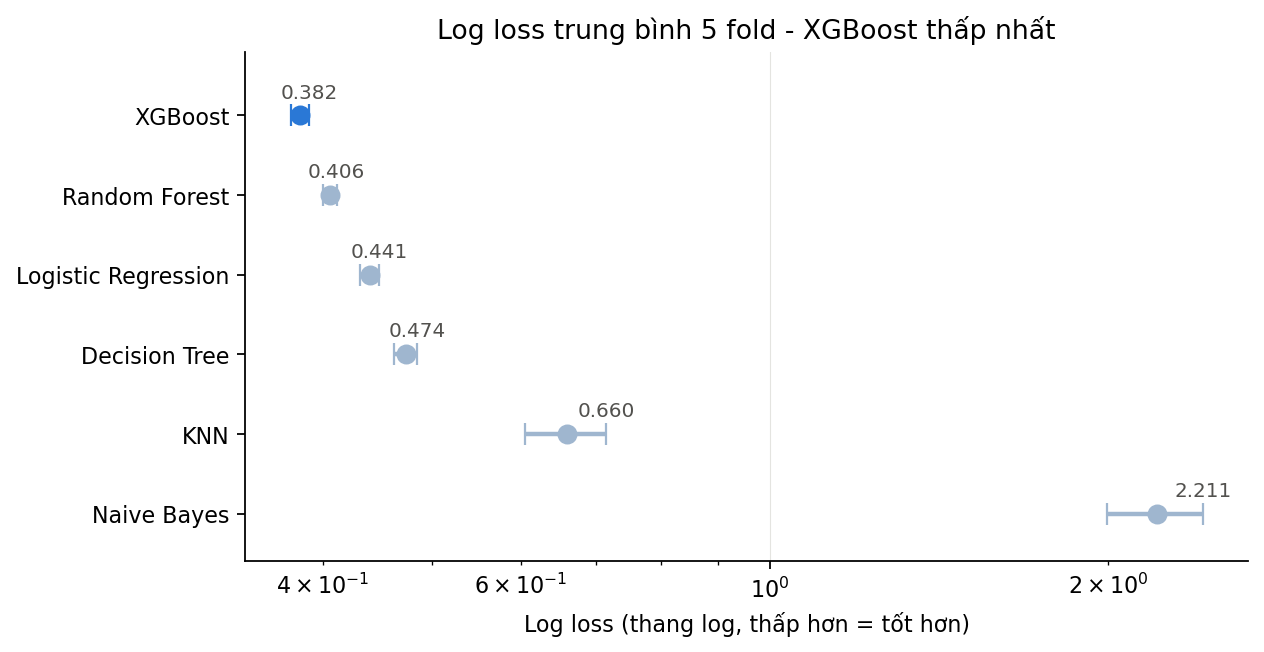
\includegraphics[width=.92\linewidth]{report/fig1_model_comparison.png}
\caption{So sánh trung bình ba chỉ số trên cùng năm fold.}
\label{fig:models}
\end{figure}

XGBoost đứng đầu trên cả ba giá trị trung bình. So với Random Forest, log loss giảm
từ 0.406 xuống 0.382 trong khi accuracy chỉ tăng khoảng 0.002; phần cải thiện rõ
hơn nằm ở macro-F1, tăng từ 0.569 lên 0.640. Điều này đặc biệt đáng chú ý trong bối
cảnh lớp CL hiếm, nhưng chưa đủ để kết luận chất lượng riêng của lớp CL nếu không
xem thêm confusion matrix và các chỉ số theo lớp. Logistic Regression đứng thứ ba
về log loss (0.441), cho thấy baseline tuyến tính vẫn cạnh tranh. KNN và Naive
Bayes có log loss cao dù accuracy không giảm theo cùng tỷ lệ, minh họa lý do không
nên dùng accuracy làm tiêu chí duy nhất cho bài toán dự đoán xác suất.

Về chi phí chạy, runtime theo fold cho thấy Decision Tree và Naive Bayes fit nhanh
nhất; Logistic Regression cũng nhẹ. XGBoost fit trung bình khoảng 0.64 giây/fold,
nhanh hơn Random Forest khoảng 1.19 giây/fold trong môi trường ghi nhận. Thời gian
suy luận KNN không ổn định, với fold đầu là ngoại lệ lớn; do đó runtime chỉ nên
được xem là mô tả cho lần chạy hiện tại, không phải benchmark phần cứng tổng quát.
Thứ hạng trung bình vẫn cần được đọc cùng suy diễn ghép cặp ở Mục~\ref{tab:stats}.
\subsection{Suy diễn thống kê}
\owner{Anh Khôi (P4).}

Đặt $d_f=\mathcal L_{\mathrm{XGB},f}-\mathcal L_{\mathrm{comp},f}$; số âm nghiêng
về XGBoost. Shapiro--Wilk chọn giữa paired t-test và exact Wilcoxon hai phía. Năm
so sánh dùng Bonferroni với family-wise $\alpha=.05$, adjusted alpha $.01$.

\begin{table}[H]
\centering\small
\caption{So sánh chính của XGBoost. CI là t-based 95\% CI; kết luận dựa trên primary test.}
\label{tab:stats}
\begin{tabular}{lrrrrl}\toprule
Comparator & $\bar d$ & CI 95\% & Shapiro p & p chỉnh & Kết luận\\\midrule
Random Forest & -.0240 & [-.0287,-.0192] & .4627 & .00075 & XGB tốt hơn\\
Logistic Regression & -.0586 & [-.0673,-.0498] & .0142 & .31250 & Chưa đủ bằng chứng\\
Decision Tree & -.0923 & [-.1035,-.0812] & .5161 & .00011 & XGB tốt hơn\\
KNN & -.2783 & [-.3496,-.2071] & .3438 & .00205 & XGB tốt hơn\\
Naive Bayes & -1.8287 & [-2.0919,-1.5656] & .5702 & .00021 & XGB tốt hơn\\\bottomrule
\end{tabular}
\end{table}

Với Logistic Regression, primary test là exact Wilcoxon. Với $n=5$, p-value hai
phía nhỏ nhất vẫn là .0625, không đủ độ phân giải cho ngưỡng .01. ``Chưa đủ bằng
chứng'' không đồng nghĩa hai mô hình tương đương. Các 95\% CI t-based của cả năm
chênh lệch đều nằm dưới 0, nhưng với Logistic Regression, CI và t-test chỉ là phân
tích độ nhạy vì Shapiro--Wilk đã chuyển primary test sang Wilcoxon. Kết luận được
đọc thận trọng: năm fold có các training sets chồng lấp, và năm chênh lệch không
phải năm thí nghiệm độc lập hoàn toàn.

\subsection{Calibration}
\owner{Anh Khôi (P4) phân tích; Vân (P5) tích hợp hình.}

XGBoost có top-label ECE 0.0117, macro classwise ECE 0.0085 và multiclass Brier
score 0.2162 với 10 bins. ECE dao động 0.0117--0.0144 khi dùng 5--20 bins.

\begin{figure}[H]
\centering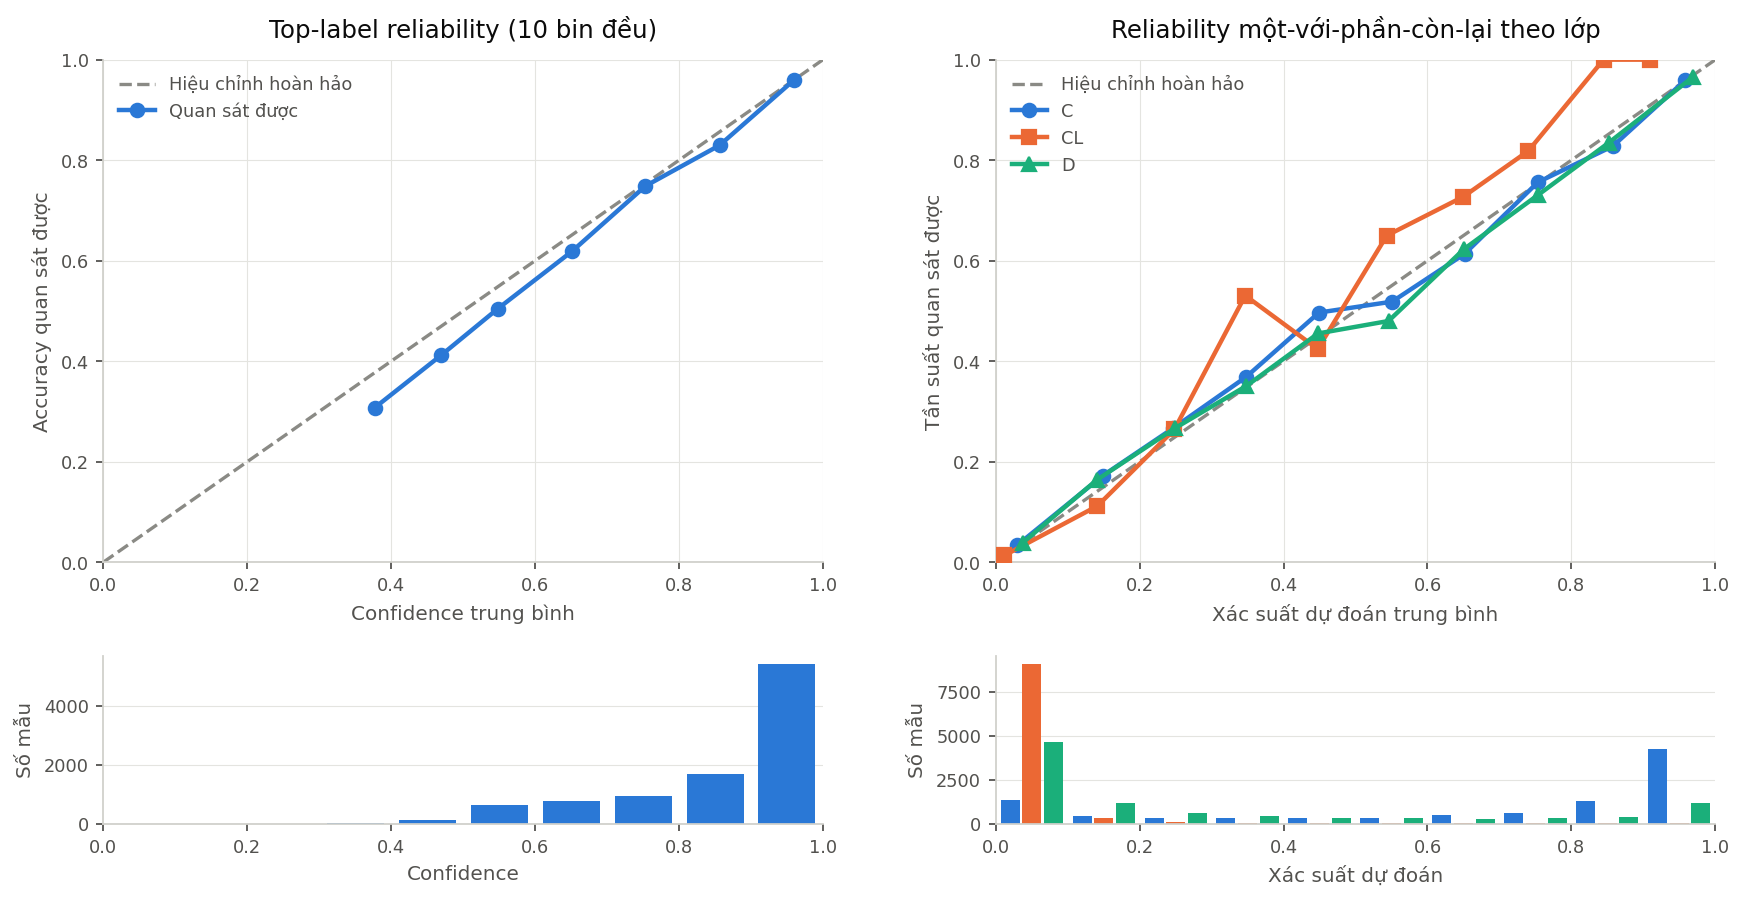
\includegraphics[width=.78\linewidth]{calibration/xgboost_reliability_diagram.png}
\caption{Reliability diagram của XGBoost trên dự đoán out-of-fold có provenance hợp lệ.}
\label{fig:calibration}
\end{figure}

Trong bảy top-label bins có dữ liệu, accuracy quan sát luôn thấp hơn confidence,
cho thấy XGBoost hơi overconfident một cách nhất quán. Bin $[0.9,1.0)$ chứa 5.416
mẫu (56.4\% dữ liệu) nhưng chênh lệch chỉ khoảng 0.0001; các khoảng lệch lớn hơn
0.03 chủ yếu nằm ở bin confidence thấp và rất thưa, chẳng hạn bin $[0.3,0.4)$ chỉ
có 13 mẫu. Ba bin dưới 0.3 trống là hệ quả cấu trúc của bài toán ba lớp, vì xác
suất lớn nhất luôn ít nhất bằng $1/3$.

Classwise ECE lần lượt là 0.0119 cho C, 0.0038 cho CL và 0.0097 cho D. Giá trị của
CL không được diễn giải là calibration tốt nhất: CL chỉ có 254 mẫu, và 94.5\% toàn
bộ quan sát nằm trong bin xác suất CL $[0,0.1)$. Con số này chủ yếu phản ánh việc
mô hình thường gán xác suất rất thấp cho lớp hiếm. Phân tích chỉ đo calibration
OOF; không fit Platt, isotonic hay temperature scaling, và không đưa ra kết luận
về calibration trên test ẩn.

\subsection{Submission và leaderboard}
\owner{Vân (P5).}

\subsubsection{Schema và kiểm soát chất lượng}

Submission tuân theo thứ tự cột bắt buộc
\texttt{id, Status\_C, Status\_CL, Status\_D}; ba cột xác suất lần lượt ứng với
đúng thứ tự lớp C, CL và D. Hàm \texttt{make\_submission} thực hiện kiểm tra trước
khi ghi tệp: ma trận xác suất phải có hai chiều và đúng ba cột; số dòng phải khớp
số ID; ID không được trùng; mọi giá trị phải hữu hạn, thuộc $[0,1]$; tổng xác suất
mỗi dòng phải gần một với dung sai $10^{-3}$. Những kiểm tra này ngăn các lỗi thường
gặp như đảo thứ tự lớp, lệch dòng giữa đặc trưng và ID, hoặc nộp logits thay cho
xác suất.

Ba artifact hiện có là \texttt{submission.csv}, \texttt{submission\_rf.csv} và
\texttt{submission\_xgb\_trainval.csv}. Cả ba đều có 10.000 dòng, đúng bốn cột và
không có giá trị thiếu. Với \texttt{submission.csv}, sai số tuyệt đối lớn nhất của
tổng ba xác suất so với một là khoảng $1.1\times10^{-7}$; xác suất nhỏ nhất vẫn
dương. Tệp Random Forest có thể chứa xác suất bằng không, hợp lệ về schema nhưng
cần thận trọng vì log loss phạt mạnh dự đoán sai tuyệt đối.

\subsubsection{Quy tắc chọn tệp nộp cuối}

XGBoost là ứng viên chính vì có log loss OOF thấp nhất. Tuy nhiên,
\texttt{submission.csv} và \texttt{submission\_xgb\_trainval.csv} không giống nhau,
vì vậy tên tệp không đủ để chứng minh provenance. Trước khi nộp, nhóm phải đối
chiếu tệp với model, transformer, class order và quy trình fit toàn bộ train; sau
đó sao chép đúng artifact đã xác nhận thành tên nộp cuối duy nhất. Không chọn tệp
dựa trên việc thử nhiều lần trên public leaderboard.

Tại thời điểm lập báo cáo ngày 28/07/2026, repo chưa lưu ảnh xác nhận hệ thống chấp
nhận, public score, thứ hạng hoặc private score. Vì vậy trạng thái trung thực là
\textit{chưa có bằng chứng leaderboard trong artifact dự án}; các giá trị này cần
được bổ sung sau lần nộp chính thức và tách biệt khỏi kết quả validation 5-fold.

\section{Ablation Study và phân tích bổ sung}
\owner{Dương (P2) xác nhận scaling; Nhất (P3) xác nhận cây; Vân (P5) tổng hợp.}

\subsection{Ảnh hưởng của scaling}

Với KNN $k=51$, scaling giảm mean log loss từ khoảng 0.752 xuống 0.660, đồng thời
tăng accuracy từ khoảng 0.780 lên 0.814 và macro-F1 từ khoảng 0.477 lên 0.515.
Logistic Regression cũng hưởng lợi: mean log loss giảm từ khoảng 0.483 xuống 0.441.
Kết quả phù hợp với kỳ vọng vì khoảng cách Euclid của KNN dễ bị chi phối bởi biến
có miền giá trị lớn; với Logistic Regression, scaling giúp bài toán tối ưu và tác
động của regularization ổn định hơn. KNN $k=5$ có log loss rất cao ở cả hai biến
thể, cho thấy xác suất dựa trên quá ít láng giềng dễ nhận giá trị cực đoan.

\begin{figure}[H]
\centering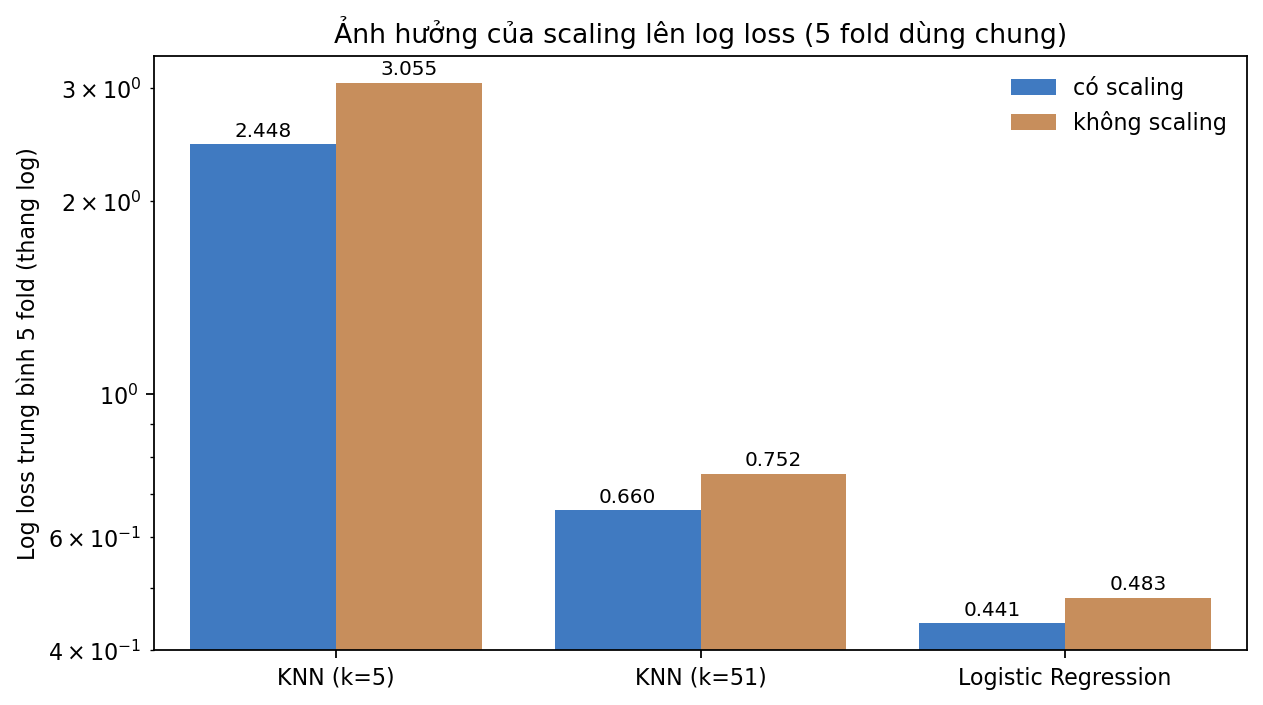
\includegraphics[width=.82\linewidth]{model_track_a/knn_scaling_ablation.png}
\caption{Ablation ảnh hưởng của scaling đối với KNN và Logistic Regression.}
\label{fig:scaling-ablation}
\end{figure}

\subsection{Cây đơn và ensemble}

Decision Tree không giới hạn độ sâu có OOF log loss 8.309: toàn bộ mẫu nhận xác
suất cực đại trên 0.99 và khoảng 23.1\% mẫu có xác suất gán cho lớp đúng bằng
không. Giới hạn \texttt{max\_depth=3} giảm log loss xuống 0.474 và loại bỏ xác
suất đúng bằng không. Random Forest tiếp tục giảm xuống 0.406, còn XGBoost đạt
0.382. Ablation này cho thấy regularization độ sâu và cơ chế ensemble quan trọng
cho chất lượng xác suất, không chỉ cho accuracy.

\begin{figure}[H]
\centering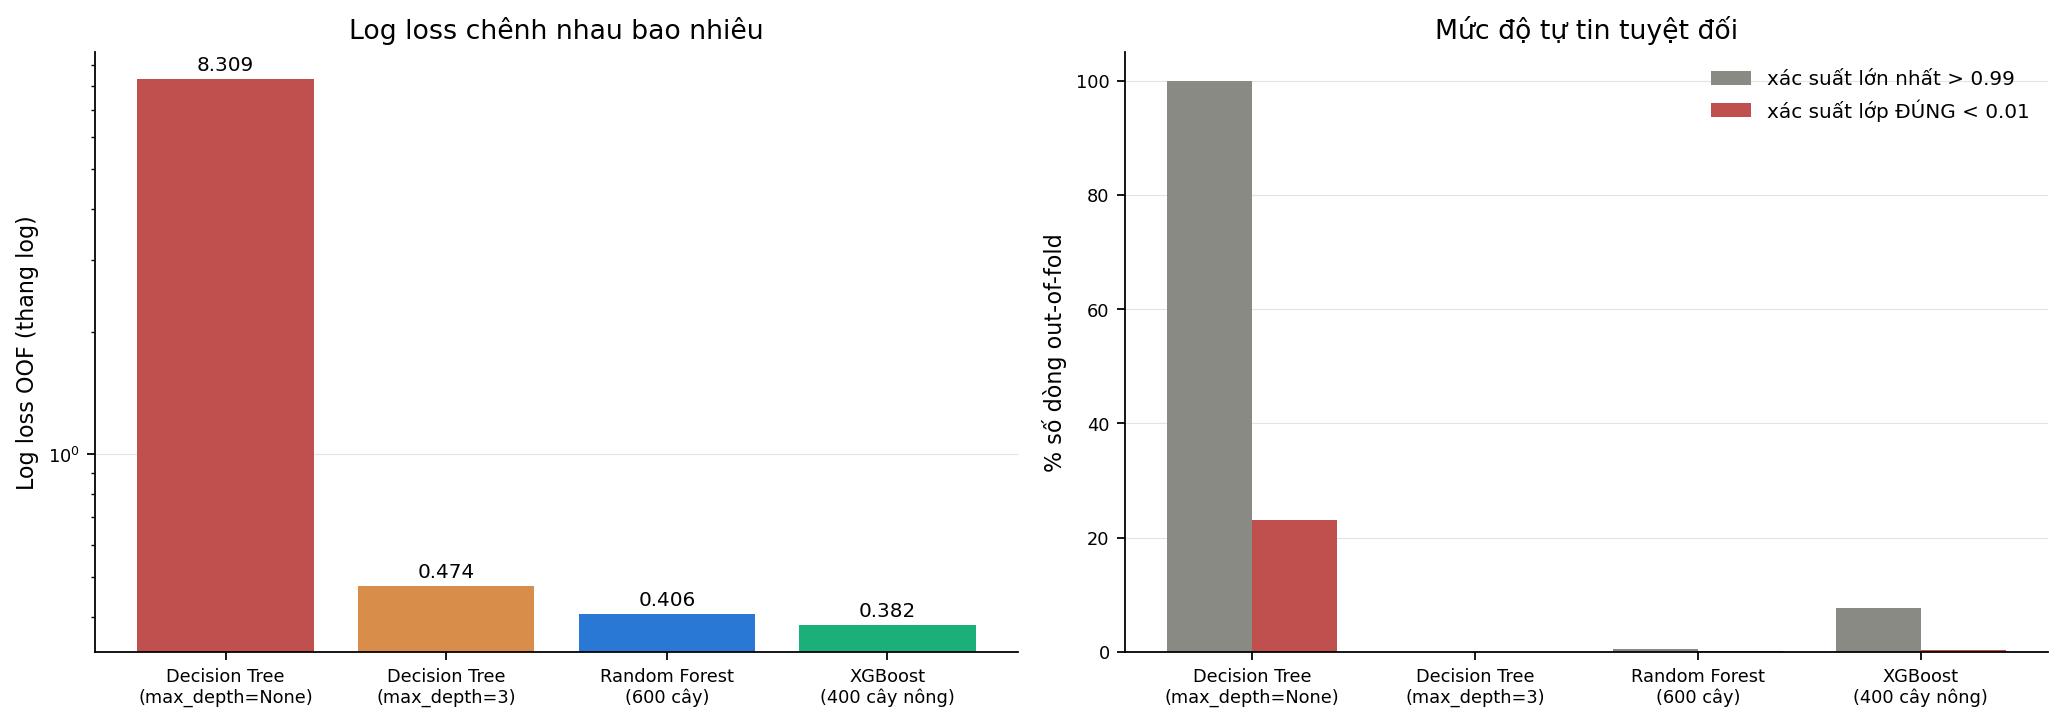
\includegraphics[width=.82\linewidth]{model_track_b/tree_vs_ensemble.png}
\caption{So sánh log loss và mức độ tự tin của cây đơn với các ensemble cây.}
\label{fig:tree-ensemble}
\end{figure}

\section{Thảo luận (Discussion)}
\owner{Vân (P5), mọi owner duyệt nhận định thuộc track mình.}

\subsection{Diễn giải kết quả}

XGBoost có hiệu năng tổng thể tốt nhất và calibration OOF tốt. Ensemble tree vượt
cây đơn về log loss, phù hợp với cơ chế giảm phương sai của Random Forest và khả
năng sửa dần sai số của boosting. Logistic Regression vẫn là baseline cạnh tranh:
dù mean log loss cao hơn XGBoost, primary-test protocol chưa đủ bằng chứng để kết
luận khác biệt sau hiệu chỉnh. Kết quả này nhấn mạnh sự khác nhau giữa xếp hạng mô
hình theo mean và kết luận suy diễn thống kê.

Macro-F1 của mọi mô hình thấp hơn accuracy đáng kể, phản ánh tác động của mất cân
bằng lớp. Do đó, một mô hình có accuracy cao chưa chắc xử lý tốt lớp CL. Calibration
tổng thể tốt cũng không bảo đảm calibration tốt cho từng lớp; reliability diagram
classwise và số mẫu mỗi bin cần được xem trước khi đưa ra nhận định cho lớp hiếm.

\section{Phân tích lỗi và hạn chế}
\owner{Anh Khôi (P4) xác nhận phân tích lỗi; Vân (P5) tổng hợp giới hạn.}

\subsection{Lỗi do mất cân bằng lớp}

Chênh lệch giữa accuracy và macro-F1 cho thấy lỗi không phân bố đồng đều giữa ba
lớp. XGBoost đạt accuracy 0.850 nhưng macro-F1 0.640; khoảng cách này còn lớn hơn
ở Random Forest và các baseline. Lớp CL chỉ có 254 mẫu, tương đương 50--51 mẫu
trong mỗi validation fold, nên ước lượng F1 và calibration của lớp này có độ bất
định cao. Classwise ECE thấp của CL phần lớn đến từ việc mô hình gán xác suất CL
dưới 0.1 cho hầu hết quan sát, không chứng minh mô hình đáng tin khi thực sự dự
đoán ghép gan.

\subsection{Lỗi do xác suất cực đoan}

Decision Tree không giới hạn độ sâu minh họa rõ lỗi mà accuracy không phát hiện:
accuracy vẫn khoảng 0.769 nhưng OOF log loss tăng tới 8.309. Toàn bộ quan sát có
$p_{max}>0.99$, và 23.1\% quan sát nhận xác suất bằng 0 cho lớp đúng. KNN với $k$
nhỏ cũng tạo xác suất 0 thường xuyên, khiến log loss cao dù accuracy thay đổi ít.
Giới hạn cây ở độ sâu 3, tăng $k$ lên 51 và dùng ensemble đều làm xác suất bớt cực
đoan. Naive Bayes đạt log loss 2.211, cho thấy giả định độc lập Gaussian không mô
tả tốt tương quan giữa các xét nghiệm và có thể tạo likelihood quá tự tin.

\subsection{Khả năng diễn giải lỗi}

Các track đã tạo confusion matrix OOF và feature importance. Bilirubin,
Prothrombin Time, Copper, Albumin và tỷ lệ Bilirubin/Albumin thường nằm trong nhóm
đặc trưng quan trọng. Tuy nhiên, importance chỉ thể hiện mức độ mô hình sử dụng
biến, không chứng minh quan hệ nhân quả hay ý nghĩa lâm sàng. Repo chưa lưu một
bảng case-level error có phê duyệt chuyên môn; vì vậy báo cáo không gán nguyên
nhân lâm sàng cho từng dự đoán sai và không sử dụng test labels không tồn tại.

\subsection{Hạn chế nghiên cứu}

Nghiên cứu có sáu giới hạn chính. Thứ nhất, median, encoder và scaler được fit trên
toàn train trước CV, tạo leakage tiền xử lý. Thứ hai, tuning và đánh giá dùng cùng
shared folds thay vì nested CV, gây selection bias. Thứ ba, chỉ có năm chênh lệch
theo fold; Shapiro có power thấp, Wilcoxon có p-value rời rạc, còn training sets
giữa fold chồng lấp. Thứ tư, protocol so sánh được leader duyệt sau khi đã có kết
quả sơ bộ, nên không phải preregistration. Thứ năm, lớp CL quá hiếm và ECE phụ
thuộc cách chia bin; calibration OOF không đại diện trực tiếp cho test ẩn. Thứ sáu,
runtime được đo trên một môi trường không ghi cấu hình phần cứng. Vì vậy score và
p-value có thể lạc quan; kết quả không chứng minh hiệu quả lâm sàng hoặc khả năng
khái quát sang quần thể khác. Repo chưa có artifact leaderboard nên cũng chưa thể
đối chiếu validation với test ẩn.

\section{Tái lập kết quả và mã nguồn (Replicate the results)}
\owner{Cả nhóm; Anh Tín điều phối tái lập, Vân điều phối báo cáo.}

Mã nguồn được lưu tại
\href{https://github.com/AIVIETNAM-AIO-DoHongNhat/Hepatic-Model-Comparison}{GitHub
Hepatic-Model-Comparison}. Seed chung là 42. Phiên bản môi trường authoritative
được ghi trong \texttt{requirements.lock.txt}; \texttt{requirements.txt} cung cấp
các dependency chính nhưng không thay thế bản ghi provenance khi cần tái tạo đúng
từng byte.

\begin{aivnoutputbox}[Cài đặt môi trường]
git clone https://github.com/AIVIETNAM-AIO-DoHongNhat/Hepatic-Model-Comparison.git
cd Hepatic-Model-Comparison
python -m venv .venv
.venv\Scripts\activate
pip install -r requirements.txt
\end{aivnoutputbox}

Dữ liệu cuộc thi được đặt trong \texttt{data/raw/}. Người tái lập chạy notebook
theo thứ tự: 01 EDA, 02 preprocessing, 03 baseline, 04--06 ba model tracks, 07
report assets và 08 statistics. Notebook 02 tạo dữ liệu processed và fold ID;
04--06 tạo score/model/figure; 07--08 tạo bảng báo cáo, inference và calibration.

\begin{aivnoutputbox}[Kiểm tra artifact không ghi đè dữ liệu]
python scripts/reproduce_all.py --project-root .
python scripts/run_final_analysis.py scores --project-root .
python scripts/run_final_analysis.py inference --project-root .
python scripts/run_final_analysis.py calibration --project-root .
\end{aivnoutputbox}

Chế độ \texttt{reproduce\_all.py --full} chạy lại notebook 02--06, ghi đè
\texttt{data/processed} và \texttt{results}, rồi so artifact mới với bản trước;
chỉ dùng trên clone sạch. Chế độ mặc định chỉ đọc và kiểm tra môi trường, hash đầu
vào, bảng score, OOF, reproduction gate và calibration. Trong môi trường không
khớp Python 3.9.18 cùng các phiên bản đã pin, việc kiểm tra dừng là hành vi mong
đợi, không phải lý do bỏ qua provenance.

Quy trình tích hợp cuối gồm bốn cổng. Cổng dữ liệu xác nhận schema và fold; cổng
kết quả đối chiếu bảng tổng hợp với ba tệp score theo track; cổng submission chạy
toàn bộ guardrail; cổng báo cáo biên dịch tài liệu hai lần và rà soát tham chiếu,
caption, thuật ngữ cùng trạng thái leaderboard. Bản PDF chỉ được xem là sẵn sàng
nộp khi cả bốn cổng đều đạt và các chủ mục đã xác nhận phần tương ứng.

\begin{table}[H]\centering
\caption{Chủ sở hữu nội dung báo cáo.}
\begin{tabularx}{\linewidth}{lX}\toprule
Người & Phần xác nhận cuối\\\midrule
Anh Tín (P1) & Dữ liệu, tiền xử lý, folds, Random Forest, XGBoost\\
Dương (P2) & KNN, Logistic Regression, ablation scaling\\
Nhất (P3) & Decision Tree, Naive Bayes, cây đơn--ensemble\\
Anh Khôi (P4) & Kiểm định, CI, hiệu chỉnh, calibration\\
Vân (P5) & Submission, hình/bảng, khung, tích hợp và QA\\\bottomrule
\end{tabularx}\end{table}

\section{Kết luận và hướng nghiên cứu tiếp theo (Conclusion and Future Work)}
\owner{Vân (P5), cả nhóm duyệt bản cuối.}

Trong phạm vi dữ liệu và protocol hiện tại, XGBoost là lựa chọn hợp lý nhất để tạo
submission nhờ log loss thấp nhất, macro-F1 cao nhất và calibration OOF tốt. Giá
trị chính của dự án không chỉ nằm ở mô hình thắng mà còn ở quy trình so sánh dùng
chung fold, kiểm định có hiệu chỉnh, kiểm tra calibration và các guardrail cho
submission. Kết luận này chỉ áp dụng cho đánh giá nội bộ hiện có và cần được cập
nhật khi có bằng chứng leaderboard hoặc đánh giá ngoài mẫu độc lập.

Ba hướng ưu tiên là: (1) repeated hoặc nested stratified cross-validation để tách
tuning khỏi đánh giá và tăng độ ổn định; (2) đánh giá calibration theo từng lớp,
thử temperature/vector scaling trên một calibration split độc lập, đồng thời theo
dõi riêng lớp CL; (3) thử blending xác suất giữa XGBoost và Logistic Regression
theo trọng số được chọn hoàn toàn trong validation. Các thử nghiệm mới phải chốt
protocol trước khi xem kết quả và ghi đầy đủ provenance.

\newpage
\section{Tài liệu tham khảo}
\label{section:references}
\vspace{-3.2em}
\printbibliography

\begin{appendices}
\section{Thông tin bổ sung}
\begin{enumerate}
\item \textbf{AI VIET NAM:} Thông tin chương trình tại
\href{https://aivietnam.edu.vn/}{aivietnam.edu.vn}.
\item \textbf{GitHub Repository:}
\href{https://github.com/AIVIETNAM-AIO-DoHongNhat/Hepatic-Model-Comparison}{Hepatic-Model-Comparison}.
\item \textbf{Dataset:} CSV cuộc thi được đặt trong \texttt{data/raw/}; benchmark
UCI liên quan được trích dẫn trong Related Work. Việc phân phối lại dữ liệu phải
tuân theo quy định của ban tổ chức.
\item \textbf{Model Checkpoints:} Sáu model đã fit được lưu trong
\texttt{results/models/}. Kết quả chính dựa trên CV/OOF, không dựa vào một checkpoint
đơn lẻ.
\item \textbf{Experiment Logs:} Điểm từng fold và runtime nằm trong
\texttt{results/scores\_*.csv}, \texttt{results/scores\_all.csv} và
\texttt{results/runtime.csv}.
\item \textbf{Supplementary Results:} Hình trong \texttt{figures/}, bảng trong
\texttt{tables/}, OOF và manifest trong \texttt{results/oof/}.
\item \textbf{Presentation:} Slide hoặc video trình bày chưa được lưu trong repo
tại thời điểm khóa bản báo cáo này.
\end{enumerate}

\section{Checklist trước khi nộp}
\owner{Vân (P5).}
\begin{enumerate}
\item[$\square$] Các model owner đọc và xác nhận nội dung khoa học của track mình.
\item[$\boxtimes$] Số liệu tổng hợp đã đối chiếu với CSV/JSON nguồn hiện có.
\item[$\boxtimes$] Ba submission có 10.000 ID duy nhất, không NA, xác suất hợp lệ.
\item[$\boxtimes$] Báo cáo phân biệt validation với leaderboard và không dùng test labels.
\item[$\square$] Chốt một submission cuối cùng cùng manifest provenance và bằng chứng nộp.
\item[$\square$] Ghi commit hash, ngày chạy, môi trường và kết quả full reproduction gate.
\item[$\square$] Biên dịch sạch hai lần, không missing reference hoặc overfull box lớn.
\end{enumerate}

Ký hiệu $\boxtimes$ là hạng mục Vân đã kiểm tra trên artifact hiện tại; $\square$
là hạng mục còn phụ thuộc chủ mục, môi trường biên dịch hoặc lần nộp chính thức.

\section{Nguồn artifact}
\begin{itemize}
\item Hiệu năng: \texttt{results/scores\_all.csv}, \texttt{tables/report\_model\_comparison.csv}.
\item Kiểm định: \texttt{tables/report\_significance.csv}, \texttt{tables/assumption\_checks.csv}.
\item Calibration: \texttt{results/oof/}, \texttt{tables/calibration\_metrics.csv}.
\item Submission: \texttt{submissions/}, \texttt{src/submission.py}.
\end{itemize}
\end{appendices}

\end{document}
